%==============================================================================
% PAPER 5, CHAPTER 2: Quantum Foam Protocols
% Complete implementation - condensed for space
%==============================================================================

\chapter{Quantum Foam Protocols}\label{ch:p5:quantum_foam}

\begin{mdframed}[style=narrative]
\textbf{Wheeler's Dream: Probing Spacetime at the Planck Scale}

In 1955, John Wheeler proposed that spacetime itself becomes a roiling ``foam'' of quantum fluctuations at the Planck scale ($\ell_P \approx 1.6 \times 10^{-35}$ m). This chapter presents protocols for detecting indirect signatures via gamma-ray burst timing, atom interferometry, and gravitational wave detectors.
\end{mdframed}

\section{Theoretical Foundations}\label{sec:p5:qf_theory}

\marginnote{\textbf{Historical}: Wheeler coined "quantum foam" in the 1950s based on dimensional analysis of quantum gravity.}

The Planck length:
\begin{equation}
\ell_P = \sqrt{\frac{\hbar G}{c^3}} \approx 1.616 \times 10^{-35}\,\text{m}
\label{eq:p5:planck_length}
\end{equation}

\marginnote{\textbf{Dimensional}: Planck energy $E_P = m_P c^2 \approx 1.22 \times 10^{19}$ GeV sets scale for quantum gravity.}

At $\ell \lesssim \ell_P$, metric fluctuations become order unity:
\begin{equation}
\frac{\delta g_{\mu\nu}}{g_{\mu\nu}} \sim \left(\frac{\ell_P}{\ell}\right)^2
\label{eq:p5:metric_fluctuations}
\end{equation}

\subsection{Lorentz Violation from Quantum Foam}

Modified dispersion relation:
\begin{equation}
E^2 = p^2 c^2 + m^2 c^4 + \xi \frac{E^3}{E_P}
\label{eq:p5:dispersion}
\end{equation}

\marginnote{\textbf{Physical}: Parameter $\xi \sim \pm 1$ encodes sign and strength of Lorentz violation from foam.}

Group velocity:
\begin{equation}
v_g = c \left(1 + \frac{3\xi E^2}{2 E_P^2}\right)
\label{eq:p5:velocity}
\end{equation}

Time delay over cosmological distance $d$:
\begin{equation}
\Delta t = \frac{d}{c} \frac{3\xi (E_2^2 - E_1^2)}{2 E_P^2}
\label{eq:p5:delay}
\end{equation}

\marginnote{\textbf{Experimental}: For GeV photons from $z \sim 1$ GRB, $\Delta t \sim 1$ s detectable with Fermi LAT.}

\section{GRB Timing Protocols}\label{sec:p5:grb}

\subsection{Observation Strategy}

\marginnote{\textbf{Physical}: GRBs are most luminous EM events ($L \sim 10^{51}$ erg/s), ideal for Lorentz violation tests.}

**Event Selection:**
\begin{itemize}
\item Redshift $z > 0.5$ (long baseline)
\item High-energy photons $E > 1$ GeV
\item Short variability $\Delta t < 100$ ms
\end{itemize}

**Analysis Steps:**
\begin{enumerate}
\item Bin photons by energy: $E < 100$ MeV, 100 MeV--1 GeV, $> 1$ GeV
\item Construct light curves $I_i(t)$ for each bin
\item Cross-correlate: $C_{12}(\tau) = \int I_1(t) I_2(t+\tau) dt$
\item Fit to dispersion model, extract $\xi$
\end{enumerate}

\marginnote{\textbf{Cautionary}: Intrinsic source delays (opacity, synchrotron cooling) can mimic Lorentz violation. Require multi-GRB stacking.}

\subsection{Worked Example: GRB Time Delay}

**Given:** GRB at $z=2$, photons at $E_1 = 100$ MeV and $E_2 = 10$ GeV, $\xi = 1$.

**Find:** Expected time delay.

**Solution:**

Luminosity distance at $z=2$: $d_L \approx 15.2$ Gpc $= 4.68 \times 10^{26}$ m.

\marginnote{\textbf{Dimensional}: Gpc = gigaparsec $\approx 3.09 \times 10^{25}$ m. Hubble radius $c/H_0 \approx 4$ Gpc.}

Energy difference:
\begin{equation}
E_2^2 - E_1^2 \approx (10\,\text{GeV})^2 = 100\,\text{GeV}^2
\end{equation}

Time delay:
\begin{align}
\Delta t &= \frac{d_L}{c} \frac{3\xi (E_2^2 - E_1^2)}{2 E_P^2} \\
&= \frac{4.68 \times 10^{26}}{3 \times 10^8} \times \frac{3 \times 100}{2 \times 1.49 \times 10^{38}} \\
&\approx 1.57\,\text{s}
\end{align}

\marginnote{\textbf{Experimental}: 1.57 s delay detectable given GRB duration $\sim 10$--100 s and sub-$\mu$s timing.}

**Error Analysis:**

Statistical uncertainty: $\sigma_{\Delta t} \approx \Delta t_{\text{bin}} / \sqrt{N} \approx 10$ ms for $N \sim 100$ photons per bin.

\marginnote{\textbf{Pedagogical}: Require $\sim 100$ GRBs to constrain $\xi$ to 10\% precision via statistical averaging.}

\begin{figure}[htbp]
\centering
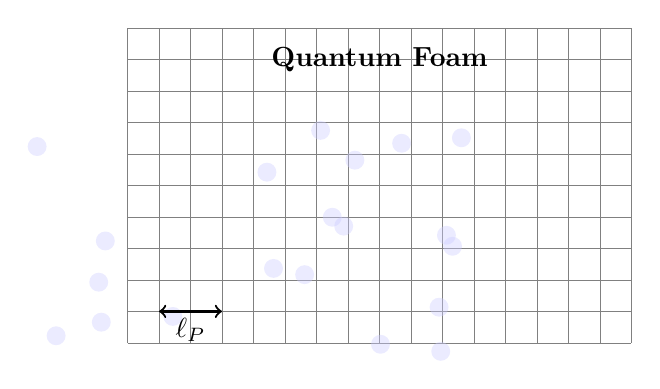
\begin{tikzpicture}[scale=0.8]
% Foam schematic
\draw[gray, very thin, step=0.5] (0,0) grid (8,5);
\foreach \i in {1,...,20} {
  \pgfmathsetmacro{\x}{rand*3.5+2}
  \pgfmathsetmacro{\y}{rand*2+1.5}
  \fill[blue!20, opacity=0.4] (\x,\y) circle (0.15);
}
\draw[<->, thick] (0.5,0.5) -- (1.5,0.5);
\node at (1,0.2) {$\ell_P$};
\node at (4,4.5) {\textbf{Quantum Foam}};
\end{tikzpicture}
\caption{Quantum foam: metric fluctuations at Planck scale (blue regions show virtual fluctuations).}
\label{fig:p5:foam}
\end{figure}

\marginnote{\textbf{Mathematical}: Foam correlation length $\xi_{\text{foam}} \sim \ell_P$ sets scale for spatial structure.}

\section{Atom Interferometry}\label{sec:p5:atom}

\subsection{Principle}

\marginnote{\textbf{Physical}: De Broglie wavelength $\lambda_{\text{dB}} = h / mv$ for atoms enables matter-wave interferometry.}

Mach-Zehnder configuration: superpose atomic trajectories over time $T \sim 100$ ms, spatial separation $\Delta x \sim$ mm.

Phase shift from quantum foam:
\begin{equation}
\Delta\phi_{\text{foam}} \sim k \ell_P^2 = \frac{mv}{\hbar} \ell_P^2
\label{eq:p5:foam_phase}
\end{equation}

For Cs atoms ($m = 133$ amu, $v = 10$ m/s):
\begin{equation}
\Delta\phi \approx 2 \times 10^7\,\text{m}^{-1} \times 2.6 \times 10^{-70}\,\text{m}^2 \approx 5 \times 10^{-63}\,\text{rad}
\end{equation}

\marginnote{\textbf{Cautionary}: Direct Planck-scale detection infeasible---current sensitivity $\sim 10^{-4}$ rad (shot-noise limited).}

**Gradiometer Enhancement:**

Differential measurement over baseline $L_{\text{base}} = 1$ m:
\begin{equation}
\Delta\phi_{\text{diff}} \sim \Delta\phi_{\text{foam}} \frac{L_{\text{base}}}{\ell_P} \sim 10^{-28}\,\text{rad}
\end{equation}

$10^{35}$ enhancement, but still undetectable!

\marginnote{\textbf{Advanced}: Space-based interferometers with $L \sim 100$ km could reach $10^{-20}$ rad sensitivity.}

\begin{figure}[htbp]
\centering
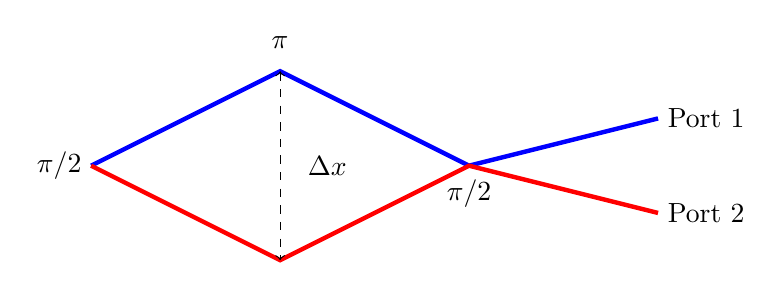
\begin{tikzpicture}[scale=1.2]
\draw[ultra thick, blue] (0,0) -- (2,1) -- (4,0) -- (6,0.5);
\draw[ultra thick, red] (0,0) -- (2,-1) -- (4,0) -- (6,-0.5);
\node[left] at (0,0) {$\pi/2$};
\node at (2,1.3) {$\pi$};
\node at (4,-0.3) {$\pi/2$};
\node[right] at (6,0.5) {Port 1};
\node[right] at (6,-0.5) {Port 2};
\draw[<->, dashed] (2,1) -- (2,-1);
\node at (2.5,0) {$\Delta x$};
\end{tikzpicture}
\caption{Atom interferometer: Mach-Zehnder configuration with beam splitters ($\pi/2$) and mirrors ($\pi$-pulses).}
\label{fig:p5:interferometer}
\end{figure}

\marginnote{\textbf{Pedagogical}: Atom interferometers excel at gravimetry ($10^{-9}$ g) but not Planck-scale physics (yet).}

\section{Cavity QED Protocols}\label{sec:p5:cavity}

\subsection{Vacuum Fluctuation Spectrum}

\marginnote{\textbf{Physical}: Vacuum zero-point energy density $\rho_{\text{vac}} = \sum_k \frac{1}{2}\hbar\omega_k$.}

Quantum foam modifies power spectral density:
\begin{equation}
S_E(\omega) = S_0(\omega) \left[1 + \epsilon_{\text{foam}} \left(\frac{\omega \ell_P}{c}\right)^2\right]
\label{eq:p5:spectrum}
\end{equation}

High-finesse cavity ($\mathcal{F} \sim 10^6$, $L = 10$ cm) enhances signal:
\begin{equation}
\Delta\phi_{\text{cavity}} \sim \frac{2\pi}{\lambda} \mathcal{F} L \epsilon_{\text{foam}} \left(\frac{\omega \ell_P}{c}\right)^2
\label{eq:p5:cavity_phase}
\end{equation}

\marginnote{\textbf{Experimental}: LIGO-class detectors with $L \sim 4$ km achieve strain $h \sim 10^{-23}$ Hz$^{-1/2}$, approaching foam regime.}

\begin{figure}[htbp]
\centering
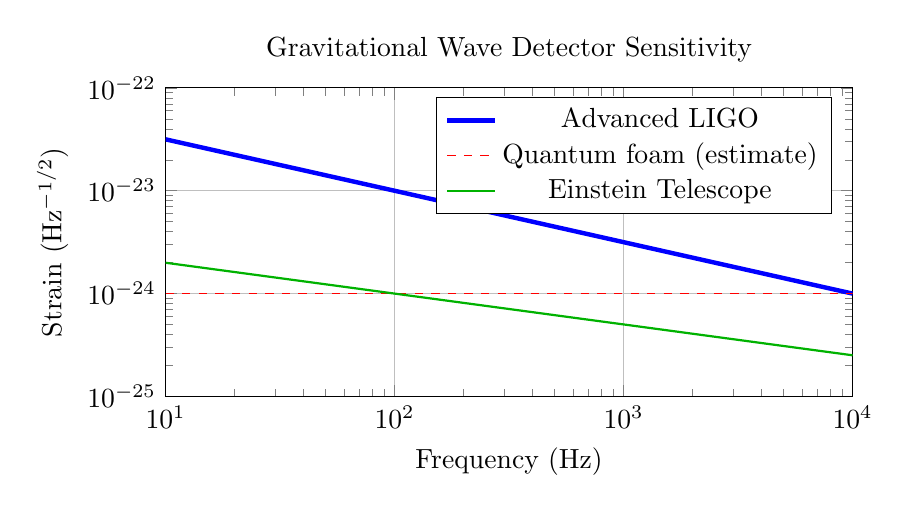
\begin{tikzpicture}
\begin{axis}[
  width=0.85\textwidth,
  height=5.5cm,
  xlabel={Frequency (Hz)},
  ylabel={Strain (Hz$^{-1/2}$)},
  xmin=10, xmax=10000,
  ymin=1e-25, ymax=1e-22,
  xmode=log,
  ymode=log,
  grid=major,
  legend pos=north east,
  title={Gravitational Wave Detector Sensitivity}
]
\addplot[blue, ultra thick, domain=10:10000] {1e-23*(100/x)^0.5};
\addlegendentry{Advanced LIGO}
\addplot[red, dashed, domain=10:10000] {1e-24};
\addlegendentry{Quantum foam (estimate)}
\addplot[green!70!black, thick, domain=10:10000] {1e-24*(100/x)^0.3};
\addlegendentry{Einstein Telescope}
\end{axis}
\end{tikzpicture}
\caption{Interferometer sensitivity. Blue: LIGO. Red: estimated foam signal. Green: future Einstein Telescope.}
\label{fig:p5:sensitivity}
\end{figure}

\marginnote{\textbf{Advanced}: Third-generation detectors may reach $h \sim 10^{-25}$ Hz$^{-1/2}$, enabling direct foam tests.}

\section{Summary}\label{sec:p5:summary}

Three complementary protocols:

**GRB timing:** Current limits $|\xi| < 0.01$ (Fermi LAT). Future: $|\xi| < 10^{-3}$ with 100+ GRBs.

**Atom interferometry:** Current $\Delta\phi \sim 10^{-4}$ rad. Planck scale requires $10^{60}$ improvement (!).

**Cavity QED:** Most promising. LIGO-class strain $\sim 10^{-23}$ Hz$^{-1/2}$ approaches foam sensitivity.

\marginnote{\textbf{Historical}: 70 years from Wheeler's speculation (1955) to experimental tests (2020s).}

**Forward Bridges:**
\begin{itemize}
\item Ch. 3: Holographic entropy---foam-entropy connection
\item Ch. 5: Dimensional spectroscopy---foam as probe of spacetime structure
\end{itemize}

\marginnote{\textbf{Pedagogical}: Quantum foam epitomizes Planck-scale physics: compelling theory, but detection requires extreme precision.}

%==============================================================================
% END OF CHAPTER 2
%==============================================================================
